%%%%%%%%%%%%%%%%%%%%%%%%%%%%%% -*- Mode: Latex -*- %%%%%%%%%%%%%%%%%%%%%%%%%%%%
%%% al_pos.tex --- 
%%% Author          : blehr
%%% Created On      : Sun Mar 28 02:27:59 1993
%%% Last Modified By: blehr
%%% Last Modified On: Sun Apr 11 18:30:30 1993
%%% RCS revision    : $Revision: 1.11 $ $Locker:  $
%%% Status          : In writing....
%%%%%%%%%%%%%%%%%%%%%%%%%%%%%%%%%%%%%%%%%%%%%%%%%%%%%%%%%%%%%%%%%%%%%%%%%%%%%%

\section{Determining the Position of the Pupil}
\label{algo:pos}

The principle behind the line oriented edge detection algorithm
employed in {\octopus} was given a fairly thorough presentation in
Section~\ref{eval:approach:edge}.  Thus the focus in this section is
on the different application specific aspects of the general
algorithm.  In Section~\ref{algo:pos:operation}, an operational
description of how line oriented edge detection has been tailored to
suit the specific needs of {\octopus} is given, and in
Section~\ref{algo:pos:operators}, the gradient operators employed to
detect the pupil contour are presented.  In Section~\ref{algo:pos:O},
the number of operations required to determine the position of the
pupil is derived.

\subsection{Operational Description}
\label{algo:pos:operation}

The original formulation of line oriented edge detection, as stated in
Section~\ref{eval:approach:edge}, says that the algorithm operates by
proceeding, from the origin of operation, in different directions,
applying some edge detecting operator successively on every pixel
encountered in each direction, and, if an edge point is recognized,
registering the coordinates of this point.  By registering the
coordinates of the oppositely positioned edge points along two
perpendicular detection lines, an estimate for the position of the
pupil can be computed using the procedure illustrated in
Fig.~\ref{fig:compute}.  By taking the average of several estimates
thus computed, an improved estimate of the position is obtained.
Accordingly, as stated in the basic formulation of the {\octopus}
algorithm in Section~\ref{eval:approach:algo}, line oriented edge
detection must be applied to as high a number of line pairs as needed
to arrive at an overall estimate that does not change from one
iteration to the next.

\subsubsection{The Direct Approach}

The normal approach to tracing a line in the discrete {\em xy\/}-plane
is to choose one parameter, say $x$, as the {\em running parameter\/},
and then solve for the other parameter, in this case $y$, by using the
general slope-intercept equation $y=ax+b$.  Which parameter to choose
as the running parameter depends on the slope $a$ of the line to be
traced; if $-1\leq a\leq 1$, $x$ is used, otherwise $y$ is used; this
is to ensure the connectivity of the traced line.  Thus, in the
general case, performing line oriented edge detection along a pair of
perpendicular detection lines involves one addition and one
multiplication, respectively one subtraction and one division for each
value taken on by the running parameters $x$ and $y$, in order to
compute the location $(x_{i},y_{i})$ of the pixel to which to apply
the edge detection operator.

If $(x_{o},y_{o})$ designates the origin of operation, an approach to
implementing the general formulation above would be to displace the
origin of the image plane by a vector $[x_{o},y_{o}]^{T}$, thus making
it coincide with the origin of operation and making all detection
lines intercept at $(0,0)$ in the transposed image coordinate system.
This would make it possible to represent each perpendicular pair of
detection lines by a single constant, namely the slope $a$ of one of
them.  The slope $a'$ of the other would be given by $a'=1/a$, and the
intercepts of both detection lines with the $y$ axis would be 0.  On
this basis, a set of detection line pairs can be maintained by
defining an array of slopes varying from 0 to $\infty$, which
corresponds to rotating the detection lines 90 degrees, thus in
principle covering all possible directions.  The actual resolution of
the directions contained in the array depends directly on its size.
An estimate of the pupil position can be computed by picking a slope
$a$ from the array, using its magnitude to determine whether $x$ or
$y$ is to be the running parameter, and then performing line oriented
edge detection along the pair of detection lines that corresponds to
$a$.  Since this procedure should be repeated until the overall
estimate no longer changes from one iteration to the next, it is
important that the number of elements in the slope array be high
enough to allow this.

There are a number of objections to this approach, despite its being a
direct implementation of Step 2 of the basic algorithm formulation.
For one, the computations necessary to obtain the coordinates of each
point along the detection lines impose a computational overhead which,
if possible, should be avoided.  Secondly, and most important, the
slope-intercept representation of straight lines is unable to express
vertical lines, and near-vertical lines have slopes with very high
magnitudes, which, in addition to being cumbersome to handle, decrease
the computational accuracy.  Thus it would be desirable with a
technique having all the advantages of the above approach, but without
the drawbacks.

\subsubsection{Repositioning the Origin of Operation}

\insertpdfwidth{lines}{\label{fig:lines}Detection lines along which
  positions do not need be computed.}{0.35}

The only way to avoid the computational overhead described above, is
to reduce the number of detection lines to four.  The only four
detection lines along which no computations are necessary to obtain
the positions are the ones occupying the horizontal, vertical and two
diagonal directions, as shown in Fig.~\ref{fig:lines}.  For the
horizontal line only the $x$ parameter is varied, for the vertical
only the $y$ parameter, and for the two diagonal lines both parameters
are varied simultaneously so that either $x=y$ or $x=-y$.  

As is seen, these lines form only two pairs of perpendicular detection
lines, thus reducing the number of estimates for the pupil position to
two.  Evidently, an overall estimate computed from only two iterations
of line oriented edge detection will not suffice to satisfy the
requirement of accuracy---particularly since the procedure should
continue to iterate until the overall estimate no longer changes from
one iteration to the next.  Apparently, however, with the given origin
of operation, no more iterations are possible without returning to the
direct approach which was deemed not satisfactory above.  There is,
however, an obvious solution to this problem: Perform the two first
iterations, obtain an overall position estimate and move the origin of
operation to this estimated position.  Thus another two iterations can
be made, resulting in an improved overall estimate.  This procedure
is, as for the above procedure, repeated until a final overall
estimate is obtained.  In fact, the only principal difference in
operation between the above technique and this, assuming that the
``quality'' of an estimate is constant with respect to the location of
the origin of operation in the image, is that with the latter, the
origin of operation has to be updated every second iteration.

The process of iterating the above procedure until an overall position
estimate has been found may, if the intermediate estimates for some
reason are distributed over a relatively large portion of the pupil,
cause the available time interval of 20 ms to be exceeded without
having arrived at a final overall position estimate.  To avoid this
happening, an upper limit to the number of iterations can be
determined.  This number has to determined on the basis of the time
required to perform one iteration\footnote{\label{pg:iterationtime}In
  the current implementation, this number is set to 55, given that
  each iterations requires $\sim 0.35$ ms (cf.
  Section~\ref{algo:eval:test}).  The lowest number of iterations
  required to arrive at a final overall estimate for all test images
  is 5.}.  If it should happen that the allowed number of iterations
has been carried out without having arrived at a final overall
estimate, the current estimate has to be returned.  Clearly, the
estimate thus returned would hardly satisfy the requirement of
accuracy.  However, assuming a relatively good image quality and thus
minimizing the spatial distribution of the intermediate estimates, the
probability of this happening will practically be zero.

Note that, when combining an intermediate position estimate with the
current overall estimate to obtain an improved overall estimate, the
current overall estimate has to be weighted according to the number of
intermediate estimates that contribute to it.  Otherwise, if the
``improved'' estimate were computed as the average of two equally
weighted image positions, one being the overall and the other being an
intermediate estimate, all the contributions made to the overall
estimate by previous intermediate estimates would be lost, and a
situation could occur in which the origin of operation is moved around
in the pupil without ever settling at a final position.  This also
applies to the direct approach above.

\subsubsection{Skipping the ``Dead Region'' about the Origin of
  Operation}
\label{pg:dead}

\insertpdfwidth{dead}{\label{fig:dead}The shaded region designates a
  portion of the pupil lake, and the white circle designates the
  ``dead region'' about the origin of operation, inside which the
  sought pupil contour will not be found.}{0.28}

If the image quality is relatively good, that is, when choosing a
reasonable value for $T_{l}$, the extent of the pupil lake corresponds
fairly close to the actual extent of the pupil and does not extend
beyond the actual pupil contour, there is a way of reducing the time
needed for one iteration of the above procedure.  Recall how the
initial origin of operation is supplied by the swimming octopus search
algorithm.  Evidently, if $T_{s}\approx 1$ (cf.\ 
Section~\ref{algo:seek:octopus}, p.~\pageref{pg:Ts}) and the above
requirement of the pupil lake not extending beyond the actual pupil
contour is satisfied, an origin of operation cannot be supplied that
lies closer to the pupil contour than $r_{d}=r_{o}/\sqrt{2}$.  This is
illustrated in Fig.~\ref{fig:dead}.  The shaded region designates a
fraction of the (idealized) pupil lake, and the white circle
designates a ``dead region'' about the origin of operation inside
which the probability of locating the pupil contour is zero.  Thus,
when moving outwards along the detection lines, looking for the pupil
contour, the initial $r_{d}$ pixels of the horizontal and vertical
detection lines and the initial $r_{d}/\sqrt{2}$ pixels along the
diagonal detection lines can be skipped, reducing the overall number
of locations at which to apply the edge detection operators.

With low-contrast images, however, like the given test images, the
``dead region'' may not be entirely ``dead''.  In other words, the
initial origin of operation may lie closer to the actual pupil contour
than $r_{d}$.  This can be attributed to the fact that $T_{s}$ has to
be chosen relatively low to ensure that some actual pupil point are
recognized as such.  Since the pupil lakes in low-contrasted images
tend to have ponds dispersed around them, some of which may lie on the
outside of the pupil boundary (cf.\ Section~\ref{algo:seek:octopus}),
there is a probability that the octopus will settle at a location at
which it has one or even two of its arms crossing the pupil boundary.
This happens when it jumps to a location at which the first
swim-criterion is satisfied by its having one (or two) of its hands in
a non-pupil pond.  Consequently, by skipping the assumed ``dead
region'', one may happen to start looking for the pupil boundary after
actually having crossed it, thus never finding it.  One solution to
this problem would be to try to choose a smaller value for $r_{d}$.
It is, however, not clear which criteria to use when choosing this
smaller value, since nothing is known about the distribution of the
non-pupil ponds surrounding the pupil lake.  Consequently, the
recommended solution, and the one I chose, since the probability of
this happening was relatively high with the given test images, is to
set $r_{d}=0$.

\subsubsection{Skipping Lake Pixels}
\label{pg:skiplakepixels}

A way of reducing the time required for one iteration of the above
procedure even further, assuming that the pupil lake does not extend
beyond the actual pupil contour, is, during the process of moving
along the detection line, to investigate whether or not the pixel {\em
  in front\/} of the current pixel is wet.  If it is dry, the edge
detection operator is applied at the corresponding location.  However,
if it is wet, there is no need to apply the edge detection operator at
this location, since the pupil contour will not be detected at a
location where both the pixel at the location and the pixel in front
of it in the direction of movement are wet.  The pixel at the given
location is known to be wet since, with this technique, every pixel in
the direction of movement is tested for wetness, so that when testing
a given pixel for wetness, it is known that all pixels preceding it
are wet.  After a dry pixel has been detected, the edge detection
operator is applied to every pixel along the remaining portion of the
detection line until the pupil contour is detected.

Evidently, the number of locations at which the relatively costly edge
detection operator has to be applied is drastically reduced by
employing this technique.  The largest impact of the technique is
obtained when the number of islands encountered along the detection
lines is minimal, so that the first dry pixel detected is in the
proximity of the actual pupil contour.  This corresponds to having
relatively high-contrasted images with correspondingly deep pupil
lakes.  However, also with the low-quality test images, the effect of
applying this technique was notable, and for the few images without
islands in the pupil lake (cf.\ Fig.~\ref{fig:lake}), the effect can
be characterized as dramatic.  Assuming relatively high image quality,
this effect can be attributed to the fact that the number of locations
at which the edge detection operator has to be applied is more or less
independent of the resolution $N$ of the image, whereas the number of
locations whose pixels are tested for wetness along the detection
line, a computationally cheap operation, is $O(N)$.

\subsection{Edge Detection Operators}
\label{algo:pos:operators}

\insertpdf{profile}{\label{fig:profile}(a) The profile of a pixel row 
  in an image. (b) The result of applying the mask in
  Fig.~\protect\ref{fig:sobelop}(b) to this profile.}

In the basic algorithm formulation in
Section~\ref{eval:approach:algo}, it was said that, based on the
comparison of different spatial edge detection schemes in
Fig.~\ref{fig:compare}, some sort of first-order derivative operator
would be best suited for the task of detecting the pupil contour.  Two
obvious candidates are the Sobel operators described in
Section~\ref{image:edge:gradient} and shown in Fig.~\ref{fig:sobelop}.
The result of applying these to Fig.~\ref{fig:testimages}(e) is shown
in Fig.~\ref{fig:compare}(c).  Although the pupil contour is hardly
discernible in the original image, it is clearly visible in the
processed image.  Thus, by moving along the detection lines
originating at the current origin of operation and at each pixel
appropriately thresholding the output from the Sobel operators, the
pupil contour can be detected.

\subsubsection{Characteristics of the Sobel Operators}

Before deciding to employ the Sobel operators directly as they are
depicted in Fig.~\ref{fig:sobelop}, it is necessary to examine their
characteristics and to determine if and how they can be tailored to
suit the task they are to perform.

Normally, assuming the image origin to be the upper left corner of the
image, the Sobel operators are applied to an image in two passes, one
vertical, applying the mask Fig.~\ref{fig:sobelop}(a) column by column
to every pixel in a top-down manner, and one horizontal, applying the
mask in Fig.~\ref{fig:sobelop}(b) row by row to every pixel in a
left-to-right manner.  In Fig.~\ref{fig:profile}(b), the result of
applying the horizontal Sobel operator to a single row in an image is
shown\footnote{The image in question is the one depicted in
  Fig.~\ref{fig:testimages}(b).  The selected row passes horizontally
  through the approximate middle of the pupil (cf.\ 
  Fig.~\ref{fig:landscape}).  Note that the darkest gray level in the
  unprocessed profile is 15, as pointed out earlier.  Note also that
  the contrast is relatively good in the image.  It was a general
  trend with the given test images that the horizontal contrast was
  much better than the vertical (cf.\ Fig.~\ref{fig:landscape}).}.
The profile of the row itself is depicted in
Fig.~\ref{fig:profile}(a).  Note that the processed profile in (b)
also contains information about the neighbouring rows to the row in
(a).  As is seen from the figure, the operator responds to positive as
well as negative edges.  Note in particular the high peaks caused by
the two edges of the reflection occupying the left portion of the
pupil.  The lack of differentiation between positive and negative
edges is due to the returned response being computed as the magnitude
of the actual response (corresponding to the partial gradients $G_{x}$
and $G_{y}$, cf.\ Eq.~(\ref{eq:gradient:abs}),
p.~\pageref{eq:gradient:abs}).  It should be noted that the pupil by
no means constitutes a flat surface in the image landscape.  Moreover,
the irregularities present in the pupil are interpreted as edges,
however small, by the Sobel operators, as is evident from the figure.
Thus one cannot assume the pupil contour to be the first edge
encountered along the detection lines.  Instead it has to be assumed
that the pupil contour constitutes the first edge encountered which
causes a response higher than or equal to a threshold value $T_{e}$.
The magnitude of $T_{e}$ is discussed below.

By examining the two masks in Fig.~\ref{fig:sobelop} and keeping in
mind that the mask in (a) proceeds in a top-down manner and the one in
(b) in a left-to-right manner, it is seen that a positive edge causes
a positive actual response, whereas a negative edge causes a negative
actual response.  Lastly, two points should be noted about the
coefficients employed in the masks.  For one, the 2's cause intensity
transitions in the column/row along which the mask moves to contribute
more to the overall response than transitions in the neighbouring
columns/rows.  This is clearly desirable from a line oriented edge
detection viewpoint.  Secondly, the ``empty'' (i.e., filled with 0's)
row/column of the masks lessen their sensitivity to spurious noise
from neighbouring rows/columns which intercept the column/row along
which the mask moves.

\insertpdfwidth{masks}{\label{fig:masks}Eight masks that can be used 
  to detect the pupil contour along the four detection lines in
  Fig.~\protect\ref{fig:lines}.  The central point represents the
  origin of operation.}{0.4}

\subsubsection{Tailoring the Sobel Masks}

The primary difference between the usual manner in which the Sobel
operators are applied, as described above, and the manner in which
they would be applied in line oriented edge detection, is the
direction of movement.  They would no longer move in only two
directions, top-down and left-to-right, but in eight different
directions corresponding to the four detection lines depicted in
Fig.~\ref{fig:lines}.  Evidently, the vertical mask would be well
suited to detect the northern and southern pupil edges, and the
horizontal mask would be equally well suited to detect the western and
eastern edges.  They would both be equally but not particularly well
suited to detect the diagonal edges, and thus at least two new masks
have to be designed that are better suited to this task.

Before proceeding to design the new masks, it should be noted that,
when moving from a point inside the pupil, the pupil contour will
always constitute a positive edge.  Accordingly, approximately half of
the edges encountered along the detection lines can be discarded,
namely those that are negative.  It was pointed out above that the
lack of differentiation between the responses to positive and negative
edges was due to the returned response being computed as the magnitude
of the actual response.  Thus, by not taking the magnitude of the
actual response and discarding all negative responses, only positive
edges will be detected.

By discarding all negative responses, the two masks in
Fig.~\ref{fig:sobelop}(a) and (b) can only be applied to detect the
southern and eastern pupil edge, respectively, since the northern and
western edges would cause negative responses and thus be discarded.
However, by mirroring the mask in Fig~\ref{fig:sobelop}(a) about the
horizontal axis and the one in (b) about the vertical axis, two masks
are obtained that would return positive responses to the northern and
western pupil edges, respectively.  The diagonal masks are obtained
analogously, and the entire set of eight masks, two for each detection
line, is shown in Fig.~\ref{fig:masks}.

\subsubsection{Reducing the Sensitivity to Noise}

\begin{figure}[tb]
  \makebox[0.45\textwidth][r]{
    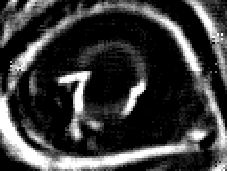
\includegraphics[width=0.3\textwidth]{figurer/dtctbl05.pdf}}
  \makebox[0.45\textwidth][l]{
    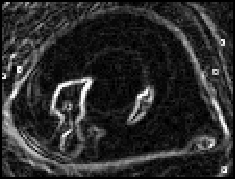
\includegraphics[width=0.3\textwidth]{figurer/soblbl05.pdf}}
  \hspace*{0.28\textwidth}(a)\hspace*{0.38\textwidth}(b)
  \caption{\label{fig:mysobel}(a) The result of
  applying the extended versions of the diagonal masks in
  Fig.~\protect\ref{fig:masks} to the image in
  Fig.~\protect\ref{fig:testimages}(e). (b) The result of applying the
  ``normal'' Sobel masks to the same image.}
\end{figure}

%\inserttwopdf{dtctbl05}{soblbl05}{\label{fig:mysobel}(a) The result of
%  applying the extended versions of the diagonal masks in
%  Fig.~\protect\ref{fig:masks} to the image in
%  Fig.~\protect\ref{fig:testimages}(e). (b) The result of applying the
%  ``normal'' Sobel masks to the same image.}

As has been stated earlier, the given test images have low contrast
and are also infected with additive, spurious noise.  Particularly
should the dark ``spots'' dispersed throughout the images be noted
(cf.\ Section~\ref{algo:intro:images})\footnote{These ``spots'' can be
  seen as negative peaks in the image landscape in
  Fig.~\ref{fig:landscape}, and are also visible in the images
  themselves, cf.\ Fig.~\ref{fig:testimages}.}.  Since the combination
of low contrast and spurious noise may cause edges to be detected
where no edge should be detected, it is important to reduce the
spurious noise in the image as much as possible, at least inside the
pupil, since this is where the edge detection takes place.
In particular must the dark ``spots'' be more or less eliminated,
since these would cause the Sobel operators to detect veritable
``walls'' if they should happen to be located along or next to the
detection lines.

An obvious approach to more or less eliminating the irregularities
inside the pupil, as well as the spots, is to process the
lake-thresholded image instead of the raw image itself.  As stated
earlier (cf.\ Section~\ref{algo:seek:idea}), lake-thresholding an
image causes sub-lake landscape features to be eliminated, whereas the
features of non-lake regions are preserved.  By appropriately choosing
the lake-threshold value $T_{l}$, the probability of having the pupil
lake extend beyond the actual pupil contour can be reduced to a
minimum, albeit with low-quality images it cannot entirely be
eliminated.  Consequently, all sub-lake ``edges'' will be ignored by
the edge detection operators and the first edge detected will
correspond to the shore of the pupil lake, alternatively to the shores
of an island in the lake.  By appropriately thresholding the output
from the operators, it is possible to differentiate between these
edges and the actual pupil edge, assuming that the pupil edge is the
most prominent of these.  Most importantly, the dark ``spots'' will
also be ``filled'', and thus either form small, one-pixel ponds of
their own, or be part of larger lakes.

With the given test images, the number of islands in the pupil lake
was on the average relatively high, and on occasions fooled the edge
detection operators into believing that the pupil edge had been
detected.  A way of reducing the operators' sensitivity to this kind
of regional noise is to enlarge the neighbourhood over which they
compute the gradient.  That is, the $3\times 3$ neighbourhoods in
Fig.~\ref{fig:masks} are extended to (e.g.) $5\times 5$ masks by
inserting two rows and two columns containing only 0's between the
three existing rows and columns.  Since the inserted 0's do not
contribute to the computation, doing this does not increase the number
of operations needed to compute the gradient at a given location, but,
since pixel values are gathered from a larger neighbourhood, it
reduces the sensitivity of the masks to islands in the pupil lake and
to spurious noise in general.  $5\times 5$ versions of $3\times 3$
masks will in the following be referred to as {\em extended\/}.  The
result of applying the extended versions of the diagonal masks in
Fig.~\ref{fig:masks} to the image in Fig.~\ref{fig:testimages}(e),
applying each mask according to which quadrant of the image relative
to the origin of operation the pixel in questions belongs to, is shown
in Fig.~\ref{fig:mysobel}(a), together with the result of applying the
standard Sobel masks of Fig.~\ref{fig:sobelop} to the same image (b).
Note that the pupil contour is more predominant in (a) than in (b),
and also that negative edges as seen from the origin of operation are
not visible (note in particular the far side of the reflection).

\subsubsection{Thresholding the Output from the Sobel Operators}

\insertpdf{myprofil}{\label{fig:myprofile}(a) The profile of the image 
  in Fig.~\protect\ref{fig:testimages}(d) along a north-eastwards
  detection line passing through the pupil. (b) The result of applying
  the SW and NE Sobel mask of Fig.~\protect\ref{fig:masks} to this
  profile.  $O_{O}$ designates the origin of operation.}

Evidently, the ability to differentiate between the pupil edge and
spurious intensity variations in the proximity of the pupil edge
depends on how the output from the employed Sobel operators is
thresholded.  With the given test images, the S/N ratio is so low that
it often is difficult on the basis of an image profile visually to
determine where the actual pupil contour is.  This is clearly
demonstrated in Fig.~\ref{fig:myprofile}(a), which shows the profile
of the image in Fig.~\ref{fig:testimages}(d) along a north-eastwards
detection line passing through the pupil.  Although the pupil lake is
clearly identifiable, this is not the case for the southwestern pupil
contour (left of the pupil lake).  Note the two islands in the pupil
lake, and that the southwestern shore constitutes a {\em plain\/}
whose height above the lake level is only 1.  Note also that this
plain, apart from three {\em hills\/} of height 2, extends almost to
the margin of the eye.  In Fig.~\ref{fig:myprofile}(b) is shown the
result of applying the extended southwest and northeast masks of
Fig.~\ref{fig:masks} to this profile.  $O_{O}$ designates the origin
of operation.  Note that the processed profile also contains
information about neighbouring lines to the actual detection line, as
can be seen from the hill ``ranges'' on both sides of the pupil lake,
as well as from the two ``extra'' islands by the northeastern shore.

Clearly, the detected extent of the pupil along this detection line
depends heavily on the threshold value $T_{e}$.  Particularly,
choosing $T_{e}$ too high would cause one or both of the actual pupil
edges along the given detection line to remain undetected.  Moreover,
the edges detected and assumed to represent to the pupil contour would
actually represent the more prominent edges at the margins of the eye.
Furthermore, choosing $T_{e}$ too low would cause the edges of the
islands in the pupil lake to be recognized as representing the pupil
contour.  As is seen from the figure, the interval of appropriate
values for $T_{e}$ can be very narrow, depending on the image
quality\footnote{\label{pg:TEproblems}With the given test images, it
  was impossible to choose a value for $T_{e}$ which was appropriate
  for all images.  $T_{e}=5$ was found to be the best overall choice.
  However, as is seen from Fig.~\ref{fig:myprofile}(b), this value
  caused unwanted results in some images.}.  However, if the image
quality and in particular the contrast is relatively high, so that the
number of islands in the pupil lake is reduced to a minimum and the
slope of the pupil contour is relatively steep, it ought to be
possible to choose an overall satisfactory value for $T_{e}$.

Note that the standard deviation of the error in the obtained position
estimate caused by the given value for $T_{e}$ apparently being
inappropriate for the profile along a detection line in a given image
will approach zero as the number of iterations increase.  When the
estimate no longer changes from one iteration to the next, which is
the stop criterion for iteration process, the error is less than one
pixel with respect to the pupil contour as seen from the current
origin of operation.  Thus it is of vital importance to ensure the
highest possible image quality in the images fed to the {\octopus}
eye-tracking algorithm.  Some requirements the images ought to satisfy
in order to increase the probability of having {\octopus} return
accurate position estimates are listed in
Section~\ref{algo:eval:improve}.

\subsection{Number of Operations}
\label{algo:pos:O}

The number of operations required to obtain one intermediate position
estimate, that is, to perform line oriented edge detection four times
along two perpendicular detection lines, is determined by the number
of pixels from the origin of operation to the pupil contour along the
given detection line.  On the average, this number equals the radius
of the pupil in pixels, which in turn depends on the horizontal and
vertical resolution $N$ of the $N\times N$ image.  Since the number
$n$ of iterations necessary to arrive at a final overall position
estimate, in addition to being limited upwards, generally satisfies
the relation $n\ll N$, it can be concluded that the position
determining part of the {\octopus} eye-tracking algorithm performs in
$O(N)$ time.  It should be noted, however, that, by applying the
technique of skipping lake pixels, described in
Section~\ref{algo:pos:operation}, p.~\pageref{pg:skiplakepixels}, the
number of locations in the image at which the edge detection operators
have to applied is reduced to $O(1)$.
